\subsection{LiDAR Sensoren}
LiDAR-Sensoren sind ein essenzielles Instrument in der modernen Sensorik, welche erm�glichen, pr�zise Messungen der Umgebungen zu erstellen. 
Die einfachsten Sensoren bestehen aus einem Time-of-Flight (TOF) Distanzmesser, welches einen Lichtpuls sendet und die Zeit misst, die es f�r die R�ckkehr ben�tigt. 
Die LiDAR Sensoren werden grunds�tzlich in 3 Kategorien aufgeteilt:

\textbf{1D-LiDAR}
In seiner grundlegendsten Form besteht der LiDAR-Sensor aus einem Distanzmesser, der seine Reichweite in einer einzigen Dimension misst. 
Dieser Ansatz erm�glicht eine schnelle Erfassung von Entfernungen entlang einer Linie, was als 1D-LiDAR bekannt ist. 
Die Genauigkeit dieser Messungen h�ngt von verschiedenen Faktoren ab, wie der Leistung des Laserimpulses, der Empfindlichkeit des Photosensors und der Rotationsgeschwindigkeit der Basis. 
Diese Ger�te sind im Handwerk verbreitet und haben bei geringen Kosten eine hohe Genauigkeit.

\textbf{2D-LiDAR}
Durch die kontinuierliche Rotation des Distanzmessers um eine Achse wird der 1D-LiDAR zu einem 2D-LiDAR erweitert. 
Diese Erweiterung erm�glicht eine Erfassung von Entfernungen entlang einer Linie und gleichzeitig um die eigene Achse herum. 
Dadurch entsteht eine 2D-Karte der Umgebung, die eine detailliertere Darstellung erm�glicht. 
Diese Ger�te sind mechanisch komplex, da der Sensor im Idealen Fall bei exakt gleich bleibender Geschwindigkeit genau horizontal gedreht werden muss. 
Diese Sensoren sind bei autonomen Ger�ten im Indoor-Bereich verbreitet, wie zum Beispiel ein Saug-Roboter oder ein autonomes Lieferfahrzeug in einer Lagerhalle.

\begin{figure}[H]
    \centering
    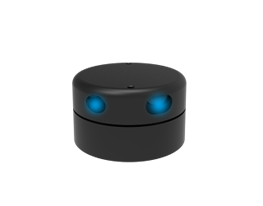
\includegraphics[scale=0.55]{./3_Stand_der_Technik/Abbildungen/symbolfoto_lidar_C_YDLIDAR.png}
    \caption{Symbolfoto 2D LiDAR Sensor, YDLiDAR G2 \cite{YDLiDAR2024}}
\end{figure}

\textbf{3D-LiDAR}
Ein weiterer Fortschritt in der LiDAR-Technologie ist der 3D-LiDAR, der nicht nur um eine Achse rotiert, sondern auch in der H�he verstellbar ist. Durch diese zus�tzliche Dimension werden bestimmte H�hen nacheinander abgetastet, wodurch eine vollst�ndige dreidimensionale Punktwolke der Umgebung erstellt wird. Diese Ger�te haben entweder mehrere gestapelte Sensoren um eine Art Punktwolke zu erstellen oder modifizieren die H�he des Lasers von einer einzelnen Quelle. Die Genauigkeit und Aufl�sung dieser Punktwolke h�ngt von der Art des Sensors sowie die Pr�zision und der Rotationsmechanik ab.

\textbf{Anwendung und Bedeutung}
LiDAR-Sensoren finden in verschiedenen Anwendungen Anwendung, darunter Gel�nde- und Geb�udevermessung sowie Unterst�tzung autonomer Fahrzeuge. Die M�glichkeit, pr�zise Entfernungen zu messen und detaillierte 3D-Karten zu erstellen, macht sie unverzichtbar f�r Projekte, die eine genaue Umgebungswahrnehmung erfordern. Die Erfassung der Intensit�t des reflektierten Lichts erm�glicht zudem eine detaillierte Oberfl�chencharakterisierung, was in vielen Anwendungen von gro�em Nutzen ist.
